\documentclass[11pt]{article}
\usepackage[utf8]{inputenc}
\usepackage{graphicx}
\usepackage{titlepic}
\usepackage{caption}
\usepackage{subcaption}
\usepackage[a4paper, total={6in, 8in}]{geometry}

% \documentclass{beamer}
\usepackage{amsmath}

\newcommand{\namesigdate}[2][5cm]{%
  \begin{tabular}{@{}p{#1}@{}}
    #2 \\[0.4\normalbaselineskip] \hrule \\[0pt]
    {\small } \\[2\normalbaselineskip] 
  \end{tabular}
}

\title{\vspace*{\fill} \textbf{Automated Image Captioning}
	  \\ {\large \textbf{COD310: Mini Project}}
	  \\  \vspace{3mm} 
\includegraphics[width=5cm]{logo.jpg}}

\author{
	\textbf{Suyash Agrawal}\\ 
	2015CS10262\\
	Computer Science\\
	CGPA: 9.92 \\
	Mob: 9717060183\\
	cs1150262@iitd.ac.in
	\and
	\textbf{Madhur Singhal}\\ 
	2015CS10235\\
	Computer Science\\
	CGPA: 8.66\\
	Mob: 9540972599\\
	cs1150235@iitd.ac.in
}
\date{\textbf{Supervisor:-} \\ \textbf{Subhashis Banerjee} \\ Professor \\ Department of CSE \\ suban@cse.iitd.ac.in\\ IIT Delhi\\
\vspace*{\fill}}




\begin{document}
	\maketitle

\begin{center}
\noindent\rule{3.2cm}{0.4pt} 
\end{center}

\begin{flushright}
\noindent\rule{3.2cm}{0.4pt} 
\\ \textbf{Prof. S. Arun Kumar}
\\ Head of Department
\\ Department of CSE
\\ sak@cse.iitd.ernet.in
\end{flushright}


	\newpage

	\section{Introduction}
		\textit{\textbf{Video Description}} is the process of discovering knowledge, structures, patterns and events of interest in the video data and describing them in natural language. Video Description is an open problem in computer vision and currently the only source of video description is manual labour. 
		\newline
		Video Description has wide variety of applications. It can help visually impaired people ``see'' the world by describing the scene around them. It has also use in automated surveillance by analyzing the videos in real time and reporting malicious or unusual activities. It can also be used to efficiently index large video databases based upon their content for ease of accessibility.

		\begin{figure}[ht!]
		\centering
		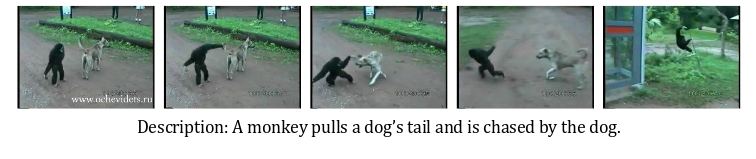
\includegraphics[width=1.0\textwidth]{description.png}
		\caption{Sample Video Description\label{fig0}}
		\end{figure}		

		Most of the prior work in this field is focused on generating natural language descriptions from images.\newline
		Our aim is to utilize these new techniques in the field of image captioning and generate natural language descriptions from video data. Basically this project will involve first encoding video data using convolutional networks and then using recurrent neural networks (specifically LSTMs) to generate descriptions of these videos. Further, we will also explore using optical flow based models to improve description of videos.


	\section{Procedure}
		
		Our main objective in this project is to make a model which describes videos. For this, we will construct a deep neural network and then train it with a large database of videos with corresponding descriptions so that our model learns to describe videos.\\
		After training our model, we will get a system in which takes video as an input and outputs a text description of the video file.\\
		The video that we are trying to describe will be taken from the datasets mentioned in section 4 . As these are datasets of videos taken from varied situations and circumstances, we believe that they will generalize well on any input video. From this, we will also be able to show that specialized video description (like surveillance) can be done given appropriate amounts of labelled data.
\section{Approach to the project}
		The basic approach is to train our model using videos that already have a description, so that our networks ``learns'' to describe videos.\\
		In order to achieve this we have broken down our problem in several parts. First, we will be implementing image captioning in order to be able to encode individual video frames in fixed-length vector representation.
		Then, we will be using our constructed image captioning network's CNN (image encoder) to encode video frames sampled at a fixed interval.
		We will then use Recurrent Neural Networks to translate this representation of video into natural language domain. This translation will be achieved by using a set of encoder and decoder RNNs. Since we are working with variable length input and output, we will specifically be using LSTMs (Long Short Term Memory Networks) for encoding and decoding purposes, as they have been proven to be excellent in machine translation and generalize very well on long data input.
		\begin{enumerate}
			\item Image Captioning
			\begin{enumerate}
				\item
					Construct a convolutional neural network (VGG/Inception V3) with pre-trained weights for object classification.
				\item
					Make an RNN (LSTM) network\cite{showandtell} that takes a encoded image (using CNN) as input and then translates the image representation into natural language text.
				\item
					Train the model on datasets like MS COCO which consists of large number of captioned images.
			\end{enumerate}
			\item Video Representation
			\begin{enumerate}
				\item
					We will first sample video at a fixed rate and convert each individual frame to a fixed length vector representation using the network trained in image captioning part.
				\item
					We will then try out different approaches of video representation like:
					\begin{itemize}
						\item
							Mean Pooling over all video frame encodings obtained to get a fixed vector representation of video\cite{proposal}.
						\item
							Using RNNs to encode this variable length video representation\cite{s2vt}.
						\item
							Using 3D CNNs to directly encode videos and use simple RNNs for description generation\cite{temporal}.
					\end{itemize}					
			\end{enumerate}
			\item Natural Language Conversion
			\begin{enumerate}
				\item
					Based on how we choose to encode our video, we will have to select appropriate architecture of LSTM to be used to decode the representation
				\begin{figure}[ht!]
				\centering
					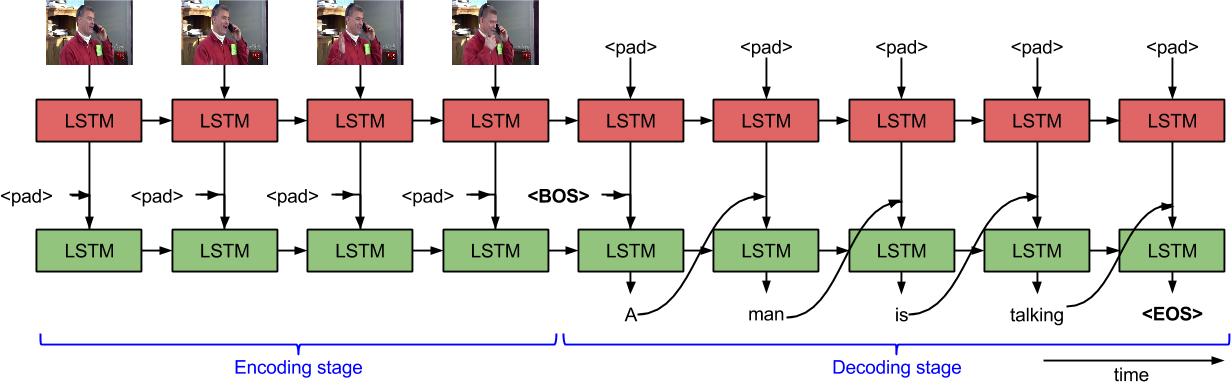
\includegraphics[width=10cm]{s2vt.png}
					\caption{Video description model with 2 LSTM levels\label{fig1}}
				\end{figure}

				\item
					One popular choice\cite{s2vt}(Figure~\ref{fig1}) that we will try out first will be to use a two level LSTM model that will do a sequence to sequence mapping from variable length video representation to variable length natural language sentence.
				\item
					Then we will train our model on the training data we have obtained and plot the learning curves.
				\item
					We will also have to check for over-fitting and under-fitting during our training process and finetune our hyper parameters according to it.
			\end{enumerate}
			\item Further Possibilities
			\begin{enumerate}
				\item We will look for techniques of data augmentation and transfer learning\cite{proposal} to compensate for the limited amount of training data for video description.
				\item We will also look into some recent techniques of using optical flow for attention modelling\cite{s2vt} which has shown in some cases to improve the results of action recognition.
				\item We will also consider using more efficient vocabulary representation as compared to one hot encoding because vocabulary in this case would be very large.
				\item Try to make forward propagation fast and more memory efficient.
				\item We will also try to develop an end user application that will speak out description of a video that a person records.
				\item A future extension of this project is to design a system which can answer questions based upon a video, similar to \cite{visualqa}.
			\end{enumerate}
		\end{enumerate}

	

	\section{Working}
		Image captioning model basically consists of two broad models:
		\begin{enumerate}
		\item
			\textbf{Image Encoder}: A deep CNN network (Inception V3) to encode images to fixed length vector representation.
		\item
			\textbf{Sequence Decoder}: An LSTM network to decode the encoded information in form of description.
		\end{enumerate}
		\subsection{Image Encoder}
			Image encoder is basically a deep CNN network pretrained on image classification dataset (ImageNet). This was chosen because CNNs are state-of-art models for object recognition and as image description relies heavily on object recognition, it became an apparent choice. Also, as these were pretrained on large object classification datasets, it was certain that they are very well optimised and are able to gather high level information from images and thus are suitable for encoding images to fixed length vector.
		\subsection{Sequence Decoder}
			LSTM were used as sequence decoders. This is so because LSTM have been very successful in tackling the problem of keeping long term dependencies and deal well with problem of exploding and vanishing gradients. Basically this unit took a fixed length vector (encoded image) as input and gave out a complete sentence that represented that input.\\
			These underlying process that is followed is:
			\begin{subsubsection}{Training Process}
				\begin{enumerate}
				\item Encoded image is fed into LSTM network to inform it about the contents
				\item A special start symbol is fed into LSTM to mark the start of sentence.
				\item For each word in our dictionary, LSTM unit gives a probability of it being the first word of our predicted caption.
				\item Then first word from the correct caption is given as input to LSTM unit and LSTM outputs the probability for second word.
				\item We then recursively do this procedure until we consume our whole caption.
				\item The loss is then calculated as sum of negative log probabilities of prediciting correct word at each step above.
				\end{enumerate}
			\end{subsubsection}
			\begin{subsubsection}{Inference Process}
				\begin{enumerate}
				\item Encoded image is fed into LSTM network to inform it about the contents
				\item A special start symbol is fed into LSTM to mark the start of sentence.
				\item For each word in our dictionary, LSTM unit gives a probability of it being the first word of our predicted caption.
				\item We take the word with highest probability as our first word and feed it into LSTM to get second word
				\item We then recursively do this procedure until we get special END word as output or we reach max length.
				\item The caption generated is basically just the sequence of predicted words by our LSTM.
				\end{enumerate}
			\end{subsubsection}
		\subsection{Overall Model}
			\subsubsection{Training}
				\begin{itemize}
				\item An image and caption pair is fetched from training dataset
				\item Image is fed into Image Encoder network to generate encoded vector.
				\item This vector along with correct caption is fed into Sequence Decoder network to get loss.
				\item This loss is backpropagated in neural network so that it can "learn" from process.
				\end{itemize}
			\subsubsection{Inference}
				\begin{itemize}
				\item Test image is fed into Image Encoder network to generate encoded vector.
				\item This vector fed into Sequence Decoder network which generates a set of captions.
				\item No backpropagation happens in this case as we don't know the correct caption and are just testing our network.
				\end{itemize}	
	\section{Results}
			\begin{itemize}
				\item
					Assisting visually impaired people to get description of their surroundings, thus enabling them to ``see''.
				\item
					Very useful for automated surveillance and theft detection by being able to analyze large amounts of data which is unfeasible to be done by humans.
				\item
					Allowing content based video retrieval by describing the contents of video in textual format which is indexable by web crawlers.
				\item
					This can also be used to detect catastrophic events through security cameras like fire breakout, murder etc.
				\item
					This project can also be applied in helping robotic vision as this project basically allows one to understand what is happening in the video and thus robots will be able to get a ``true'' sense of their surroundings.
			\end{itemize}

	\section{Future Plans}	
		\subsection{Budget}
			No budget is required for this project.			
			%Rs. 10,000 will be required for purchasing GPU instance in AWS servers as the project will require an on-demand access to very powerful GPU during training process.
			% Rs. 25,000 will be needed to purchase an android smart phone having high quality sensors and a high resolution camera.
					
		\subsection{Duration}
			We will try to complete this project by the end of the summer break i.e. the end of July, 2017. 

	\section{Background} 
			\subsection{Deep Learning}
				Deep Learning is a branch of machine learning in which multiple parameter based models are used in series. In a deep network, there are many layers between the input and output, allowing the algorithm to be executed in multiple processing steps, composed of \textbf{multiple linear and non-linear transformations}. At each layer, the signal is transformed by a processing unit, like an artificial neuron, whose parameters are \textbf{`learned'} through training. Deep Learning has been shown to excel in tasks where the goal is to find \textbf{intuitive} patterns in the data.\cite{deep} In particular, in the field of Computer Vision, deep networks are increasingly used to extract \textbf{feature descriptions and inter-relationships between features} from images.\cite{cs231n}
				\begin{figure}[ht!]
					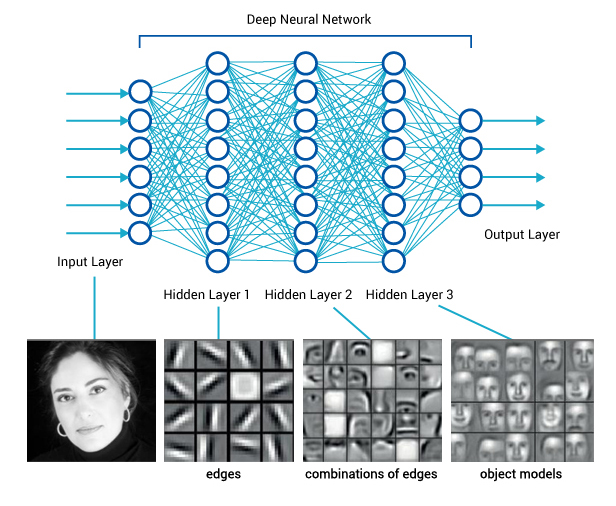
\includegraphics[width=14cm]{blog_deeplearning3.jpg}
					\caption{Illustration of Deep Learning as applied to Vision\label{fig2}}
				\end{figure}	

			\subsection{Convolutional Neural Networks}
			Convolutional Neural Networks (CNN, or ConvNet) are a type of feed-forward artificial neural network in which the connectivity pattern between the neurons is inspired by the organization of the animal visual cortex. Individual cortical neurons respond to stimuli in a restricted region of space known as the \textbf{receptive field}. The receptive fields of different neurons partially overlap such that they tile the visual field. The response of an individual neuron to stimuli within its receptive field can be approximated mathematically by a \textbf{convolution operation}. A Convolutional Neural Network consists of the following layers.\cite{showandtell}
								
				\begin{figure}[ht!]
					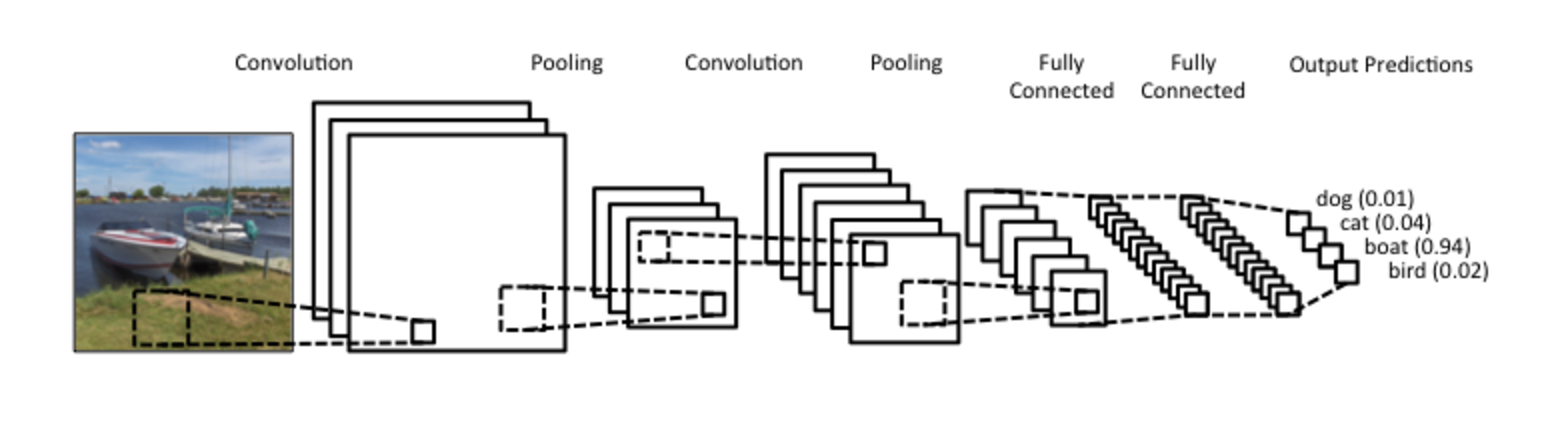
\includegraphics[width=1.0\textwidth]{conv.png}
					\caption{A Typical Convolutional Neural Network\label{fig4}}
				\end{figure}
			%skipping Relu layer since its not in picture assume it to be in conv layer
				\subsubsection{Convolutional Layer}
					The convolution layer is the core building block of a CNN. The layer's parameters consist of a set of \textbf{learnable filters} (or kernels), which have a small receptive field, but extend through the full depth of the input volume. During the forward pass, each filter is convolved across the width and height of the input volume, computing the dot product between the entries of the filter and the input and producing a $2$-dimensional activation map of that filter.\cite{cs231n} As a result, the network learns filters that activate when it detects some specific type of feature at some spatial position in the input.

				\subsubsection{Max Pooling Layer}
					It is common to periodically insert a Pooling layer in-between successive Conv layers in a ConvNet architecture. Its function is to \textbf{progressively reduce the spatial size} of the representation to reduce the amount of parameters and computation in the network, and hence to also control over-fitting. The Pooling Layer operates independently on every depth slice of the input and resizes it spatially, using the max operation.\cite{cs231n}
				\subsubsection{Fully-Connected Layer}
					Finally, after several convolutional and max pooling layers, the high-level reasoning in the neural network is done via fully connected layers. Neurons in a fully connected layer have \textbf{full connections to all activations} in the previous layer, as seen in regular Neural Networks. Their activations can hence be computed with a matrix multiplication followed by a bias offset.\cite{fullyconnected} Thus output of the fully connected layer is a vector with elements representing the `probability' (not in a strictly statistical sense) of the image containing specific objects or actions.

			\subsection{Long Short Term Memory Networks}
			    \begin{figure}[ht!]
			    	\centering
					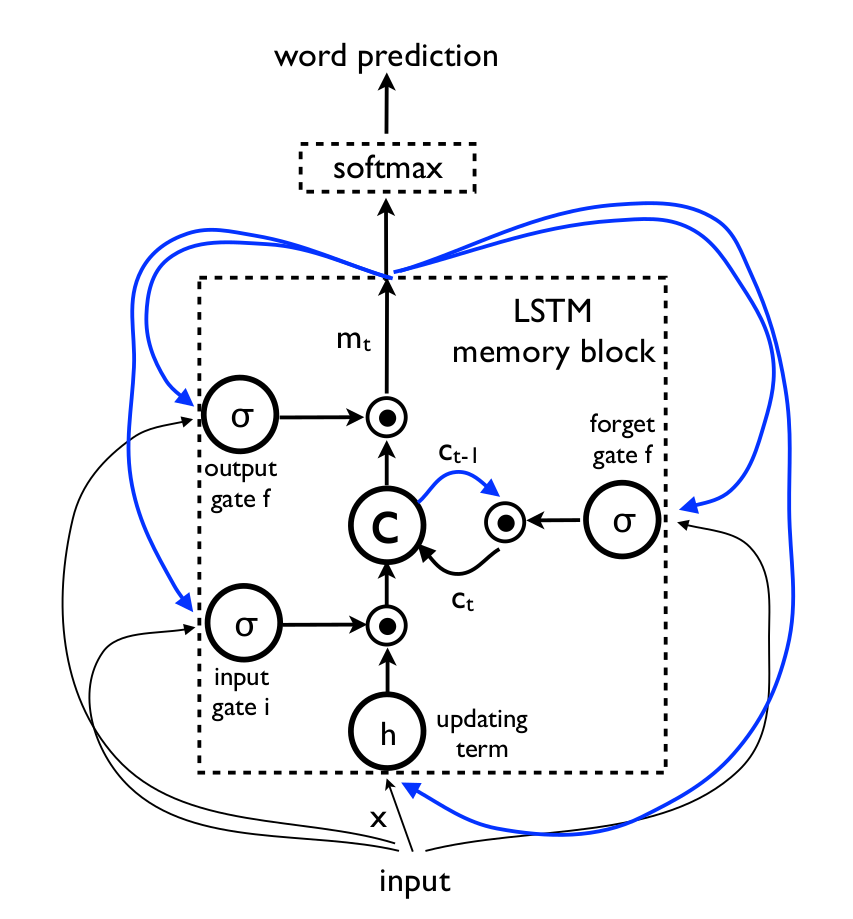
\includegraphics[scale=0.266]{LSTM_unit.png}
					\caption{A single LSTM unit\label{fig6}}
				\end{figure}
				Long Short Term Memory Networks are a type of Recurrent Neural Networks. These networks are based upon recursion, so that variable length inputs can be handled easily and sequential information can be processed with better results. LSTM's are specifically used for making RNNs learn long term patterns since traditional RNNs tend to \textbf{favour short term temporal dynamics}. It can be difficult to train traditional RNNs to learn long-term dynamics, likely due in part to the \textbf{vanishing and exploding gradients problem} that can result from propagating the gradients down through the many layers of the recurrent network, each corresponding to a particular time step\cite{ltms}. LSTMs provide a solution by incorporating memory units that explicitly allow the network to learn when to ``forget'' previous hidden states and when to update hidden states given new information\cite{lstmexecute}.\\
%				Below we list the main equations governing the behaviour of the LSTM networks.\\
%				\begin{align}
%					f_{t} &= \sigma_{g}(W_{f}x_{t} + U_{f}h_{t-1} + b_{f})\\	
%					i_{t} &= \sigma_{g}(W_{i}x_{t} + U_{i}h_{t-1} + b_{i})\\
%					o_{t} &= \sigma_{g}(W_{o}x_{t} + U_{o}h_{t-1} + b_{o})\\
%					c_{t} &= f_{t} \circ c_{t-1} + i_{t} \circ \sigma_{c}(W_{c}x_{t} + U_{c}h_{t-1} + b_{c})\\
%					h_{t} &= o_{t} \circ \sigma_{h}(c_{t})
%				\end{align}
%				The symbol meanings are:\\
%	$\mathbf{x_{t}}$: Input vector\\
%    $\mathbf{h_{t}}$: Output vector\\
%    $\mathbf{c_{t}}$: Cell state vector\\
%    $\mathbf{W}$, $\mathbf{U}$ and $\mathbf{b}$: Parameter matrices and vector\\
%    $\mathbf{f_{t}}$: Forget gate vector. Weight of remembering old information.\\
%    $\mathbf{i_{t}}$: Input gate vector. Weight of acquiring new information.\\
%    $\mathbf{o_{t}}$: Output gate vector. Output candidate\\
%    $\mathbf{\sigma_{g}}$, $\mathbf{\sigma_{c}}$ and $\mathbf{\sigma_{h}}$: Activation functions\\
		
			\subsection{Training Deep Neural Networks}
					\begin{figure}[ht!]
					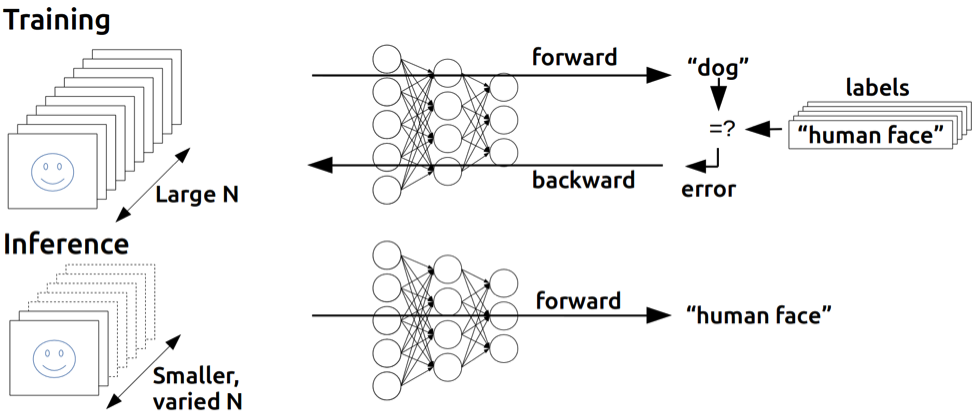
\includegraphics[width=14cm]{training_inference1.png}
					\caption{Training and Inference Processes\label{fig5}}
				\end{figure}
				A Deep Neural Network is at it's core a parameter based function. All of these parameters are  \textbf{trained} automatically from inputs and expected output tuples (training data). The training process revolves around minimizing a particular cost function using methods like \textbf{Stochastic gradient descent}. The input is given to the network in a feed forward fashion and the parameters are modified from the last layer to the first \textbf{(Backpropagation)}. Neural Networks, by design, require huge amounts of training data and take a large time to get trained. For some perspective, most current state of the art image classifiers have $> 100$ million parameters and are trained on more than 1.2 million images. 


			\subsection{Finetuning}
				Fine-tuning a network is a procedure based on the concept of
				\textbf{transfer learning}. We start training a CNN to learn features for a broad domain with a
				classification function targeted at minimizing error in that domain. Then, we
				replace the classification function and \textbf{optimize the network} again to minimize
				error in another, more specific domain. Under this setting, we are transferring
				the features and the parameters of the network from the broad domain to the
				special one.\cite{fineplant} In our project we will need to use the pre-trained image classification models 
				to actually decode individual frames of the video, thus we are planning to \textbf{fine-tune those models
				with respect to the output of our LSTMs}.



	\begin{thebibliography}{1}
	
	  \bibitem{proposal} Subhashini Venugopalan {\em Natural Language Video Description using Deep Recurrent Neural Networks}, 2015.
	
	  \bibitem{s2vt}  Venugopalan, Subhashini and Rohrbach, Marcus and Donahue, Jeff
                    and Mooney, Raymond and Darrell, Trevor and Saenko, Kate {\em Proceedings of the IEEE International Conference on Computer Vision (ICCV)}, 2015
	
	  \bibitem{showandtell} Oriol Vinyals and
               Alexander Toshev and
               Samy Bengio and
               Dumitru Erhan {\em Show and Tell: {A} Neural Image Caption Generator} 2014.

        \bibitem{lstmexecute} Wojciech Zaremba, Ilya Sutskever {\em Learning to Execute} ICLR 2015
         

         \bibitem{temporal}  Li Yao, Atousa Torabi, Kyunghyun Cho, Nicolas Ballas, Christopher Pal, Hugo Larochelle, Aaron Courville {\em Describing Videos by Exploiting Temporal Structure} ICCV 2015
        

         \bibitem{visualqa} Aishwarya Agrawal, Jiasen Lu , Stanislaw Antol,
		Margaret Mitchell, C. Lawrence Zitnick, Dhruv Batra, Devi Parikh {\em VQA: Visual Question Answering} 2016
        

         \bibitem{ltms} Jeff Donahue, Lisa Anne Hendricks, Marcus Rohrbach, Subhashini Venugopalan, Sergio Guadarrama, Kate Saenko, Trevor Darrell {\em Long-term Recurrent Convolutional Networks for Visual Recognition and Description} 2016

         \bibitem{deep} Bengio, Yoshua; LeCun, Yann; Hinton, Geoffrey {\em Deep Learning} 2015

         \bibitem{fineplant} Angie K. Reyes, Juan C. Caicedo and Jorge E. Camargo {\em Fine-tuning Deep Convolutional Networks for
		Plant Recognition} LifeCLEF 2015

         \bibitem{cs231n} Andrej Karpathy {\em 
			CS231n Convolutional Neural Networks for Visual Recognition
		} http://cs231n.github.io/convolutional-networks/

		\bibitem{fullyconnected} Santanu Chaudhury, Anupama Mallik, Hiranmay Ghosh {\em Multimedia Ontology: Representation and Applications
		} 

	\end{thebibliography}
\end{document}
